% Created 2015-12-24 Thu 04:51
\documentclass[9pt,b5paper]{article}
\usepackage{graphicx}
\usepackage{xcolor}
\usepackage{xeCJK}
\setCJKmainfont{SimSun}
\usepackage{longtable}
\usepackage{float}
\usepackage{textcomp}
\usepackage{geometry}
\geometry{left=0cm,right=0cm,top=0cm,bottom=0cm}
\usepackage{multirow}
\usepackage{multicol}
\usepackage{listings}
\usepackage{algorithm}
\usepackage{algorithmic}
\usepackage{latexsym}
\usepackage{natbib}
\usepackage{fancyhdr}
\usepackage[xetex,colorlinks=true,CJKbookmarks=true,linkcolor=blue,urlcolor=blue,menucolor=blue]{hyperref}


\lstset{language=c++,numbers=left,numberstyle=\tiny,basicstyle=\ttfamily\small,tabsize=4,frame=none,escapeinside=``,extendedchars=false,keywordstyle=\color{blue!70},commentstyle=\color{red!55!green!55!blue!55!},rulesepcolor=\color{red!20!green!20!blue!20!}}
\author{deepwaterooo}
\date{\today}
\title{Homebrew Gosu - deepwaterooo's starter game trial}
\hypersetup{
  pdfkeywords={},
  pdfsubject={},
  pdfcreator={Emacs 24.3.1 (Org mode 8.2.7c)}}
\begin{document}

\maketitle
\tableofcontents


\section{Installing Ruby, Gems, Gosu. Game Window.}
\label{sec-1}
Welcome to the first tutorial. Today we will start off from pure basics. Apart from what I have stated in the title, I will include one more thing in this tutorial - one related mainly to Ruby itself. But first things first ;)

Another thing is that I will try to explain everything in these tutorials, so people with no programming background whatsoever will be able to follow.

Let's start off with downloading and installing all we need! Let's head up to:

\begin{itemize}
\item Ruby Installer - Download Ruby 1.9.3. Do not download Ruby 2.0.0+, as at this day Gosu doesn't yet work with that version :)
\item RubyGems and download the newest version. If you are using Windows, download it in "zip" archive for Windows OS.
\end{itemize}

Additionally we may need some software to actually write out code in. There's plenty of it, even your standard Notepad will do. Some suggestions:

\begin{itemize}
\item Notepad++ is probably the most known, open editor. It's simple, and fast.
\item Aptana Studio Radrails is probably good for people that already program in Java using Eclipse, since it is pretty much Eclipse for Web Development, and Radrails is tweaked to work with Ruby on Rails. Warning: I have not used it, so I can't tell if it will work with what are we doing here.
\item Sublime Text. I use it personally, and I am really happy with it. The only offside is that it is not a free program.
\item SciTE is another good piece of software - free too! I used to work with it for quite a bit and I was happy with it.
\item Geany was recommended to me by one person, and it seems to be working on all major OS, so if you're on Linux or OSX that may be your best option.
\end{itemize}

Now, once we have everything downloaded, it's time to install it! Installing Ruby itself is easy, limited to pressing "Next" a couple of times. As for Ruby Gems and Gosu itself, it's going to be slightly more difficult.

You should immediately notice a "setup.rb" file. If you've installed Ruby correctly, you should see the same icon as I do. Double-clicking it will run setup, but Ruby has one bad thing - all programs ran in it will close immediately (with command prompt) when there's an error, giving you no time to actually read through the error. That's why you have to run it through separate Command Prompt. Hold down shift button, and right click somewhere in the folder (not on the files though!) and pick "Open command wrompt here".

Remember that, you will be using this a lot.

Once our cmd.exe is open, type in "setup.rb" and press enter. A minute or two of waiting, and you should see a note that RubyGems were installed correctly. Now what's left is installing Gosu itself. Still using our Command Prompt, type:

\lstset{language=shell,label= ,caption= ,numbers=none}
\begin{lstlisting}
gem install gosu
\end{lstlisting}

Another minute of waiting, and we should see a message saying ��1 gem installed��. That��s all, now let��s get to programming!

First, lets prepare our game folder. How you will lay it up is up to you, I have set the layout up this way:

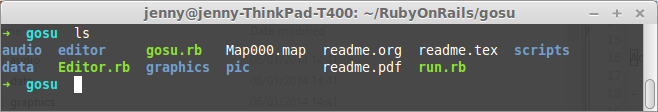
\includegraphics[width=.9\linewidth]{./pic/files.png}

In addition to that, we need a few files from Gosu folder. 

And copy everything (except 'gosu' folder) into our main game's directory. Create a new file - "Run.rb" - and open it in your chosen editor. Open up Command Window too.

Start off with creating a small note on top of the file:

\lstset{language=Ruby,label= ,caption= ,numbers=none}
\begin{lstlisting}
=begin

Project: Platformer "FuZeD"
Start date: 03/05/14
Author: Piotr Blaut ("Ekhart")

=end
\end{lstlisting}

=begin and =end marka multiline comment in Ruby. Single-line comments are marked with \#.

Before we start with creating our window, I want to say a few things about Ruby's syntax. Ruby is really open language, and syntax is not as strict as in many other languages. This means that we can write our functions in few different ways:

\lstset{language=Ruby,label= ,caption= ,numbers=none}
\begin{lstlisting}
def square(n)
return n*n
end

def square n
return n*n
end
\end{lstlisting}

And it's similar with calling our function. Both of these:

\lstset{language=Ruby,label= ,caption= ,numbers=none}
\begin{lstlisting}
square(2)

square 2
\end{lstlisting}

will work.

Ruby does not need 'return' keyword to actually return the value as well. Short functions can be written in one line, using semicolon ;. This means that this function:

\lstset{language=Ruby,label= ,caption= ,numbers=none}
\begin{lstlisting}
def square(n)
res = n*n
return res
end
\end{lstlisting}

can be written like that:

\lstset{language=Ruby,label= ,caption= ,numbers=none}
\begin{lstlisting}
def square n; n*n; end
\end{lstlisting}

and it will work too. Try it yourself!

Okay, now let's start the proper part: creating our Window. We have to import what we need first. In our 'Run.rb' file write:

\lstset{language=Ruby,label= ,caption= ,numbers=none}
\begin{lstlisting}
$: << File.dirname(__FILE__)

require 'gosu'
require 'rubygems'
include Gosu
\end{lstlisting}

From start: First line (\$: << File.dirname(\uline{\uline{FILE}})) sets this file's location as starting location. Without that line we might run into some problems with importing and using files (definitely it would be a problem in Ruby 1.8, I'm not 100\% sure about 1.9, but one line of code won't hurt you). Next thing is our require, both on 'gosu' and 'rubygems'. This loads up both libraries. And the last line, 'include Gosu', informs the system that we are using Gosu library. With this line we don't have to type in "Gosu::" whenever we're using some of Gosu's internal classes. With a large amount of libraries used, this could cause problems, but we won't use many libraries ;)

Create a new file in your Scripts folder ('/scripts' on my layout) and name it "GameWindow.rb". Open it and write:

\lstset{language=Ruby,label= ,caption= ,numbers=none}
\begin{lstlisting}
class GameWindow < Window

end
\end{lstlisting}

This creates a new class - GameWindow - which extends (uses functions of) (Gosu::)Window class. Thanks to our 'include Gosu', we didn't have to put this "Gosu::" part in front ;)

Each of our scripts will most likely need an 'initialize' method. This method is called when the script is initialized. Our window needs a few other methods as well.

\lstset{language=Ruby,label= ,caption= ,numbers=none}
\begin{lstlisting}
def initialize

end

def update

end

def draw

end

def button_down(id)

end

def button_up(id)

end
\end{lstlisting}

These methods are, as follows:

\begin{itemize}
\item update - it's called every frame (about 16 milliseconds), and it will contain all "physics" of our game.
\item draw - similarly to \#update it is called every frame. It displays everything that is put inside this method. Your computer may sometimes call this method twice in a row, so I recommend you only put displaying methods here. Small calculations (not important for game's physics) are okay too.
\item button$_{\text{down}}$ - records button press
\item button$_{\text{up}}$ - records button release
\end{itemize}

Once we've got all these methods, let's go to our \#initialize. We will need two lines of code: 'super' and 'caption'.

First method takes three parameters - width, height, fullscreen? - and creates our window. Second one "names" our window. So let's put these in:

\lstset{language=Ruby,label= ,caption= ,numbers=none}
\begin{lstlisting}
super(640,480,false)
self.caption("[Game Title]")
\end{lstlisting}

This will create a 640��480 pixels window, which will not be in full screen. It will be named "[Game Title]" (which, of course, you may change to whatever's the name of your game ;) ). Also you may have noticed 'self' in front of our caption method. This informs our computer to apply this to this specific window.

And that's all, our window's ready! Let's just type in 'Run.rb' in our Command window, press enter and\ldots{}

\ldots{}nothing. But why?!

Because we didn't do anything to actually show our window ;) it's just created, but it was not even imported, let alone initialized! So open our 'Run.rb' file and type in:

\lstset{language=Ruby,label= ,caption= ,numbers=none}
\begin{lstlisting}
window = GameWindow.new
window.show
\end{lstlisting}

window = GameWindow.new creates a new local variable named window, which is our Game Window itself. Second line calls our .show method that will display the window.

Now, once we have created our Window variable and displayed it, we can run it and see\ldots{}

Error

\ldots{}an error. That's the reason we have Command prompt open. If we were to run it by double click, we wouldn't notice the error message, as it would close immediately (check it yourself!). For now you may not know what does the error say, so let me explain. System does not recognize GameWindow. Why?

Look a couple of lines above, you will see

\lstset{language=Ruby,label= ,caption= ,numbers=none}
\begin{lstlisting}
require 'gosu'
require 'rubygems'
\end{lstlisting}

As I said earlier, this is what imports libraries and scripts. I hope you've figured it out yourself. If not, that's what we need:

\lstset{language=Ruby,label= ,caption= ,numbers=none}
\begin{lstlisting}
require 'scripts/GameWindow.rb'
\end{lstlisting}

Save and run it again, and\ldots{}

\includegraphics[width=.9\linewidth]{./pic/Window.png}

There's our window! It's completely empty\ldots{} but that's next week's tutorial :)

Hope you liked it, enjoy!


\section{Introducing Scenes. Player.}
\label{sec-2}
Welcome in the second tutorial on how to make a platformer :) today we will create our basic Scene - SceneMap, and we will make our Player character. Let's get started!

Open up the editor of your choice and both files we've created. Create a new file, name it 'SceneMap.rb' and put it into your '/scripts' folder. Remember to import it in our Run.rb file too!

\lstset{language=Ruby,label= ,caption= ,numbers=none}
\begin{lstlisting}
require 'scripts/SceneMap.rb'
\end{lstlisting}

Create the basic layout of Scene. We need few methods:

\lstset{language=Ruby,label= ,caption= ,numbers=none}
\begin{lstlisting}
class SceneMap

    def initialize

    end

    def update

    end

    def draw

    end

    def button_down(id)

    end

    def button_up(id)

    end

end
\end{lstlisting}

Each Scene will have it's own 'physics' (update queue), corresponding to correct contents, so eg. SceneTitle will have everything that's needed for a Game Title screen, and SceneMap will contain everything related to map. To make our Scene work, we have to actually create it, and call it as well. Let's switch back to our GameWindow class.

In our GameWindow\#initialize method, right under 'self.caption' we have to put this piece of code:

\lstset{language=Ruby,label= ,caption= ,numbers=none}
\begin{lstlisting}
$scene = SceneMap.new
\end{lstlisting}

This creates a new Global variable. This variable is accessible from anywhere in the program. While we're here, put this piece of code in as well:

\lstset{language=Ruby,label= ,caption= ,numbers=none}
\begin{lstlisting}
$window = self
\end{lstlisting}

This creates another global variable, window, which contains our GameWindow. We will use it later.

We also have to call \#update, \#draw and input methods in our Scenes. To do it, we have to put \$scene.[method] in each of methods in our GameWindow. It's quite simple - GameWindow\#update gets \$scene.update etc.

\lstset{language=Ruby,label= ,caption= ,numbers=none}
\begin{lstlisting}
# Main game window

class GameWindow < Window

    def initialize
        super(640,480,false)
        self.caption = "Fuzed"
        $scene = SceneMap.new
    end

    def update
        $scene.update
    end

    def draw
        $scene.draw
    end

    def button_down(id)
        $scene.button_down(id)
    end

    def button_up(id)
        $scene.button_up(id)
    end

end
\end{lstlisting}

Short explanation: since each of these methods is called automatically by our Gosu::Window class, they won't work outside of it. By putting these lines we ensure that whenever Gosu::Window has called each of these methods, corresponding Scene's method is called as well.

If you run your game now, nothing should change - we should still get black, empty window. So, how do we know if what we've done has actually worked? We don't!

Let's use one of Gosu's built-in methods to check it. Using 'Gosu::Window\#draw$_{\text{line'}}$ we will draw a straight white line inside our SceneMap class. In \#draw method of our scene, put this piece of code:

\lstset{language=Ruby,label= ,caption= ,numbers=none}
\begin{lstlisting}
$window.draw_line(0,0,Color.new(255,255,255),640,480,Color.new(255,255,255),0)
\end{lstlisting}

Again, quick explanation: we're calling in a \$window.draw$_{\text{line}}$ method. \$window is our GameWindow, but since we don't have \#draw$_{\text{line}}$ method in our class, Superclass' method is called. Works the same way as our 'self.caption'.

Gosu::Window\#draw$_{\text{line}}$ takes in 7 arguments: startX, startY, Color1, endX, endY, Color2, z. X and Y are the coordinates, and Color uses another Gosu class - Gosu::Color. 'Z' is a layer on which line lies - things displayed on higher Z value will be over the ones with lower Z. With the values we've put, we should see a line going across the window. Let's test it.

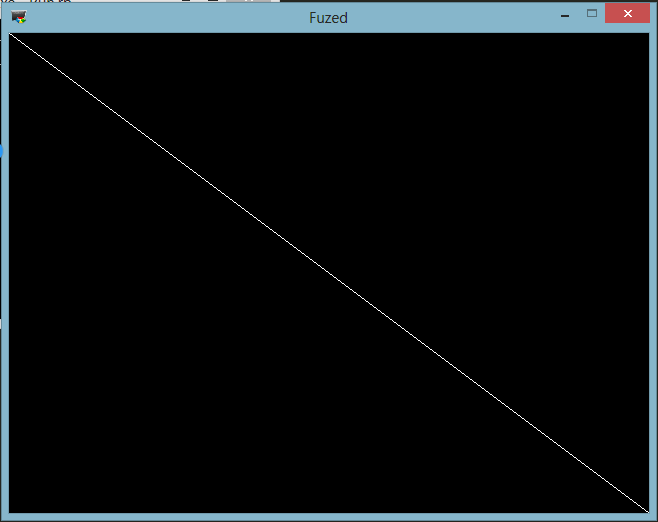
\includegraphics[width=.9\linewidth]{./pic/line.png}

So now we know that our Scene works correctly. Let's create our Player.

Create a 'Player.rb' file, put it in the '/scripts' folder, and import in Run.rb ;) At the moment we'll only need three methods in our Player class: \#initialize, \#update and \#draw. This time our \#initialize and \#draw will take in arguments. For \#initialize we're going to need x and y position of 'spawning', and for \#draw - z layer, taking a value of 5.

\lstset{language=Ruby,label= ,caption= ,numbers=none}
\begin{lstlisting}
class Player

    def initialize(x,y)

    end

    def update

    end

    def draw(z=5)

    end

end
\end{lstlisting}

As you can see, there is a small difference between the way \#initialize and \#draw takes in the arguments. In \#draw, we automatically assign a value of 5 to the local z variable. That means that if we call \#draw method without giving any arguments, we won't get any errors. \#initialize needs both arguments though.

In our \#initialize method we have to create a few variables. These are:

@x, @y, @sprite, @real$_{\text{x}}$, @real$_{\text{y}}$. The first two are simple enough. @sprite is going to hold our graphic. What about the last two? In a moment! First, lets assign the values to first two variables:

\lstset{language=Ruby,label= ,caption= ,numbers=none}
\begin{lstlisting}
def initialize(x,y)
    @x = x
    @y = y
end
\end{lstlisting}

We will create our graphic as well. I am going to provide you with resources, but by all means, if you want you can use your own graphics! If you prefer to use the same graphics as I do (at least for the time being), save this graphic into '/graphics/sprites' folder:


\includegraphics[width=.9\linewidth]{./graphics/sprites/player_1_stand_right.png}

And in \#initialize put this code:

\lstset{language=Ruby,label= ,caption= ,numbers=none}
\begin{lstlisting}
@sprite = Image.new($window, "graphics/sprites/player_1_stand_right.png", false)
\end{lstlisting}

@sprite is a new instance of (Gosu::)Image class. Image takes in three parameters - Gosu::Window (our \$window), path/to/file and a boolean (true/false value) for tile-ability. Since we won't put our character in tiles, we don't need it to be tile-able ;) let's head to Player\#draw method and draw our sprite too!

\lstset{language=Ruby,label= ,caption= ,numbers=none}
\begin{lstlisting}
@sprite.draw(@x, @y, z)
\end{lstlisting}

And viola, done! Let's create our Player on a map.

In SceneMap\#initialize create this variable:

\lstset{language=Ruby,label= ,caption= ,numbers=none}
\begin{lstlisting}
@player = Player.new(128,128)
\end{lstlisting}

This will create our Player on position \{128;128\}. You also have to use the same variable @player in \#update and \#draw methods, similarly to what we've done in GameWindow with our \$scene variable.

Now you can run your game. You should see our Player character floating somewhere in top left corner. We're doing well!

Now let's work on the remaining two variables in Player class: @real$_{\text{x}}$ and @real$_{\text{y}}$. We now have two sets of Player coordinates. I've done it this way, because we will need to save two points on our Player: @x and @y will hold the coordinates of bottom middle part of Player ('gravity center'), while their @real\_ counterparts will keep a \{0;0\} point of the sprite. We have to make a few changes in our Player\#initialize:

\lstset{language=Ruby,label= ,caption= ,numbers=none}
\begin{lstlisting}
def initialize(x,y)
    @real_x = x
    @real_y = y
    @sprite = Image.new($window, "graphics/sprites/player_1_stand_right.png", false)
    @x = @real_x + (@sprite.width / 2)
    @y = @real_y + @sprite.height
end
\end{lstlisting}

What were the changes? @x and @y were swapped with @real$_{\text{x}}$ and @real$_{\text{y}}$, then we're calculating @x and @y based on this position. We are going to need these updated in Player\#update:

\lstset{language=Ruby,label= ,caption= ,numbers=none}
\begin{lstlisting}
@real_x = @x - (@spirte.width / 2)
@real_y = @y - @sprite.height
\end{lstlisting}

As you can see, the code here is the opposite of the one in \#initialize. Now change @x and @y in \#draw to their @real\_ counterparts and run your game. Our character should now slightly move:

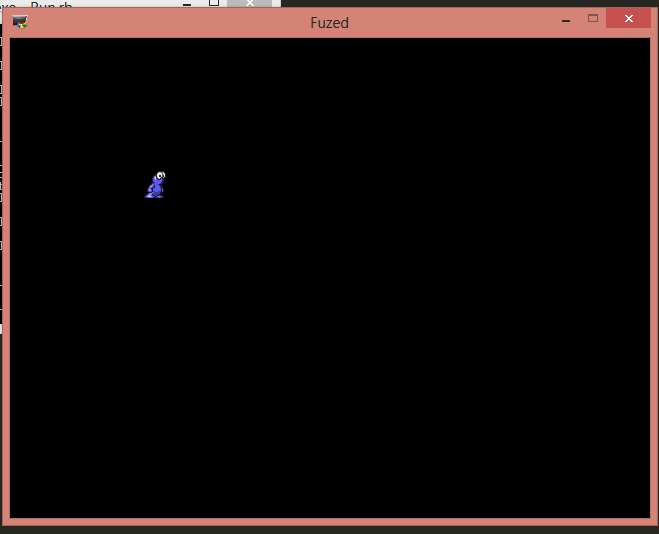
\includegraphics[width=.9\linewidth]{./pic/Player_On_Window.png}

But a static character is boring. Let's make it move!

Create another two variables in \#initialize

\lstset{language=Ruby,label= ,caption= ,numbers=none}
\begin{lstlisting}
@move_x = 0
@moving = false
\end{lstlisting}

So, how are we going to move? Every time we will call a Player's movement, the value of @move$_{\text{x}}$ will change, and @moving will switch to true. Then our \#update will react accordingly. How? This way:

\lstset{language=Ruby,label= ,caption= ,numbers=none}
\begin{lstlisting}
if @moving then
    if @move_x > 0 then
        @move_x -= 1
        @x += 1
    elsif @move_x < 0 then
        @move_x += 1
        @x -= 1
    elsif @move_x == 0 then
        @moving = false
    end
end
\end{lstlisting}

Of course this goes to Player\#update. First we have our condition: if @moving (\ldots{} is true), then call a code checking @move$_{\text{x}}$ variable. If it is greater than 0, decreases it by 1 and adds 1 to @x. If it's less than 0, it does the opposite. Finally, if @move$_{\text{x}}$ is equal to 0 (== means is equal, = only assigns value), character stops moving (@moving = false). Now create two additional methods:

\lstset{language=Ruby,label= ,caption= ,numbers=none}
\begin{lstlisting}
def move_left
    @move_x = -3
    @moving = true
end

def move_right
    @move_x = 3
    @moving = true
end
\end{lstlisting}

and let's go back to Scene\#Map. We have to call these methods in \#update once they're needed. Why in update?
Because our button$_{\text{down}}$? method is called only once, on button press, player would have to constantly press arrow buttons to actually move. So if we'll put this code:

\lstset{language=Ruby,label= ,caption= ,numbers=none}
\begin{lstlisting}
@player.move_left if $window.button_down?(KbLeft)
@player.move_right if $window.button_down?(KbRight)
\end{lstlisting}

in SceneMap\#update, it will work seamlessly on button press and hold. You can also see a second way of creating conditional if statements. It's useful when there's only single condition. Now when you'll run your game you will notice, that player finally moves around. But he's still pretty static, it would look better animated, wouldn't it?

That's what we'll do in a moment. First save this graphic:


\includegraphics[width=.9\linewidth]{./graphics/sprites/player_1_stand_left.png}

We'll start off with creating two Image variables - @stand$_{\text{left}}$ and @stand$_{\text{right}}$, and assigning a @start$_{\text{right}}$ value to @sprite:

\lstset{language=Ruby,label= ,caption= ,numbers=none}
\begin{lstlisting}
@stand_right = Image.new($window, "graphics/sprites/player_1_stand_right.png", false)
@stand_left = Image.new($window, "graphics/sprites/player_1_stand_left.png", false)
@sprite = @stand_right
@dir = :right
\end{lstlisting}

You can also notice a new Data type: Symbol (marked with a colon). Symbols are great when not used a lot, when we need a certain values assigned. Once created, Symbol cannot be edited (so we cannot change :right to :Right, it will create a new symbol and take up a bit more memory). Our @dir variable will hold two values - :right and :left. We now have to add a character rotation and sprite change. In our \#move$_{\text{right}}$ and \#move$_{\text{left}}$ methods we have to assign correct value to @dir variable. Next, in \#update, right above our 'if @moving then' put this code:

\lstset{language=Ruby,label= ,caption= ,numbers=none}
\begin{lstlisting}
if @dir == :left then
    @sprite = @stand_left
elsif @dir == :right then
    @sprite = @stand_right
end
\end{lstlisting}

This is only a temporary solution, but it works. If you'll start your game, you'll see that our character now faces the direction it's moving! Now we can start our animation. We will make a walking and standing animation. We will need these four graphics: download from \url{https://corruptgd.wordpress.com/tutorials-creating-a-platformer-in-ruby-gosu/tutorial-2-introducing-scenes-player/}

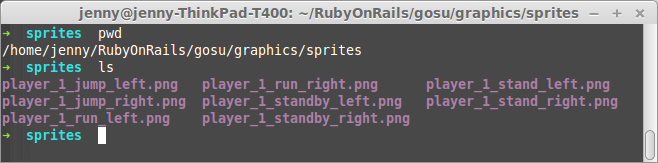
\includegraphics[width=.9\linewidth]{./pic/images.png}


As you can see, they're not exactly a one sprite, but a bunch of sprites in one graphic. Thankfully, Gosu::Image provides us with a suitable method. We will use four variables, two of which already exist: @stand$_{\text{right}}$, @stand$_{\text{left}}$, @walk$_{\text{right}}$, @walk$_{\text{left}}$. To create them we will use a Gosu::Image\#load$_{\text{tiles}}$ method, which takes 5 arguments: Gosu::Window, path/to/file, width, height, tile-ability. Width and Height are of individual sprite. Putting a negative value will divide the image by this amount (let's say putting a -4,-4 will divide our spritesheet into 16 equal sprites). Single frame of our character is 32��32 pixels, so we'll use this value:

\lstset{language=Ruby,label= ,caption= ,numbers=none}
\begin{lstlisting}
@stand_right = Image.load_tiles($window, "graphics/sprites/player_1_standby_right.png", 32, 32, false)
@stand_left = Image.load_tiles($window, "graphics/sprites/player_1_standby_left.png", 32, 32, false)
@walk_left = Image.load_tiles($window, "graphics/sprites/player_1_run_left.png", 32, 32, false)
@walk_right = Image.load_tiles($window, "graphics/sprites/player_1_run_right.png", 32, 32, false)
\end{lstlisting}

Next we have to fix our \#draw method. With these values our @sprite will now be an array of images, so attempting to draw it will cause an error. We can fix this that way:

\lstset{language=Ruby,label= ,caption= ,numbers=none}
\begin{lstlisting}
frame = milliseconds / 100 % @sprite.size
@sprite[frame].draw(@real_x, @real_y, z)
\end{lstlisting}

This will animate our sprite. Another thing is that in both \#initialize and \#update we have to change '@sprite.width/height' to '@sprite\footnote{DEFINITION NOT FOUND.}.width/height'. Now if you'll start the game, you will see our character blinking ;) you can change the speed of that blinking by changing '100' in 'frame = milliseconds / 100 \% @sprite.size' into other value. The higher the value, the slower the animation, but beware! This speed is for every Player animation we will create!

Okay, now it's time to animate our movement. It's not going to be difficult at all. First, in \#move$_{\text{left}}$ and \#move$_{\text{right}}$, change the @sprite to correct ones:

\lstset{language=Ruby,label= ,caption= ,numbers=none}
\begin{lstlisting}
def move_left
    @dir = :left
    @move_x = -3
    @sprite = @walk_left
    @moving = true
end

def move_right
    @dir = :right
    @move_x = 3
    @sprite = @walk_right
    @moving = true
end
\end{lstlisting}

Now we need our \#update code to change @sprite to @stand$_{\text{left}}$/right only when we're not moving. We're going to slightly rewrite update, so it looks like that:

\lstset{language=Ruby,label= ,caption= ,numbers=none}
\begin{lstlisting}
def update
    @real_x = @x - (@sprite[0].width / 2)
    @real_y = @y - @sprite[0].height

    if @moving then
        if @move_x > 0 then
            @move_x -= 1
            @x += 1
        elsif @move_x < 0 then
            @move_x += 1
            @x -= 1
        elsif @move_x == 0 then
            @moving = false
        end
    else
        if @dir == :left then
            @sprite = @stand_left
        elsif @dir == :right then
            @sprite = @stand_right
        end
    end
end
\end{lstlisting}

Now start the game and see our tiny alien (?) moving!

The last two things we're going to do today are falling and jumping. Let's start with falling. First we will need to create a way for SceneMap to access Player's position (since that's the class that will check if Player should be falling). To do this, we have to create 'readers' ('getters' in other programming languages) in Player class. There are two ways to do it. First is to create a

\lstset{language=Ruby,label= ,caption= ,numbers=none}
\begin{lstlisting}
attr_reader
\end{lstlisting}

above \#initialize, which will set marked variables as readable by other classes. The second one, which I prefer, is to create methods returning the values. So in our Player class, create these two methods:

\lstset{language=Ruby,label= ,caption= ,numbers=none}
\begin{lstlisting}
def get_x
    return @x
end

def get_y
    return @y
end
\end{lstlisting}

Now in SceneMap\#update add:

\lstset{language=Ruby,label= ,caption= ,numbers=none}
\begin{lstlisting}
@player.fall if no_ground?(@player.get_x, @player.get_y)
\end{lstlisting}

As you see, this line calls two methods that we don't have. Fist one is a \#no$_{\text{ground}}$?() method in SceneMap, and the other one is Player\#fall. Start off by creating a SceneMap\#no$_{\text{ground}}$? method.

It will take two parameters: x and y. Since we don't have a map yet, this method will only check if our player does not fall out of the window. So if y value we're sending is lesser than Window's height (480), we return true, otherwise we return false.

\lstset{language=Ruby,label= ,caption= ,numbers=none}
\begin{lstlisting}
def no_ground?(x,y)
    return y < 480
end
\end{lstlisting}

Obviously this method will get bigger over time ;) but now that's enough. Let's head to Player class and create a \#fall method. This method is dead simple - we're adding +2 to @y and changing the graphic.

\lstset{language=Ruby,label= ,caption= ,numbers=none}
\begin{lstlisting}
def fall
    @y += 2
    if @dir == :left then
        @sprite = @jump_left
    elsif @dir == :right then
        @sprite = @jump_right
    end
end
\end{lstlisting}

As you can see, we need two new graphics. Save these:


\includegraphics[width=.9\linewidth]{./graphics/sprites/player_1_jump_left.png}

\url{./graphics/sprites/player_1_jump_right.png }

And load them up as previous, naming them @jump$_{\text{right}}$ and @jump$_{\text{left}}$. Use Gosu::Image\#load$_{\text{tiles}}$ as well, even though they're single sprites. This will keep us from getting errors ;) Run the game:

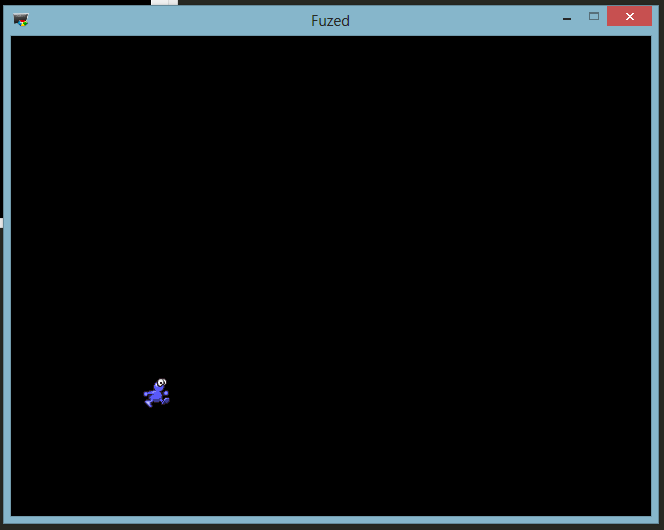
\includegraphics[width=.9\linewidth]{./pic/Player_Falling.png}

Everything is working fine. Since our player is falling now, all that's left is to make it jump! Head back to SceneMap, and in \#button$_{\text{down}}$ we'll add jump input detection. Why here and not in \#update, like we did with movement?

So the player won't 'fly'. As I said earlier, this method is called only once, on button input, so the player will have to depress and press the button again to jump once more. We have to check, if the player pressed the correct button (Arrow Up), and to see if the Player character is on ground (so we won't jump midair). At first we will just check if it works. Our \#button$_{\text{down}}$ code should look like that:

\lstset{language=Ruby,label= ,caption= ,numbers=none}
\begin{lstlisting}
if id == KbUp then
    if !no_ground?(@player.get_x, @player.get_y) then
        p "Jump!"
    end
end
\end{lstlisting}

What happens? First we check if button pressed had correct ID (KbUp). Next we make sure Player is on ground, so if our \#no$_{\text{ground}}$? method returns false (! in front of the method's name is the same as using 'not'). Alternatively we could write it as 'if no$_{\text{ground}}$?(@player.get$_{\text{x}}$, @player.get$_{\text{y}}$) == false then'.

If both of these conditions are okay, print (p) method will send a "Jump!" to our Command Window. You can check if it works (it does). Now that we're sure everything's okay, replace this print with:

\lstset{language=Ruby,label= ,caption= ,numbers=none}
\begin{lstlisting}
@player.jump
\end{lstlisting}

In Player class we'll have to create this method. But first let's create a new variable (in Player\#initialize) - @jump = 0. Then go to Player\#fall method, which we have to slightly alter and block falling while we're jumping (otherwise our character won't move at all ;) ).

\lstset{language=Ruby,label= ,caption= ,numbers=none}
\begin{lstlisting}
if @jump == 0 then
    @y += 2
    if @dir == :left then
        @sprite = @jump_left
    elsif @dir == :right then
        @sprite = @jump_right
    end
end
\end{lstlisting}

And the Player\#jump method:

\lstset{language=Ruby,label= ,caption= ,numbers=none}
\begin{lstlisting}
@jump = 15 if @jump == 0
\end{lstlisting}

This will set our @jump to 15 only if it was at 0 when we called the method.

Okay, now we've got changing @jump value, and switched off falling when @jump is over 0. Now in \#update we have to actually make player jump:

\lstset{language=Ruby,label= ,caption= ,numbers=none}
\begin{lstlisting}
if @jump > 0 then
    @y -= 5
    if @dir == :left then
        @sprite = @jump_left
    elsif @dir == :right then
        @sprite = @jump_right
    end
    @jump -= 1
end
\end{lstlisting}

What does this code do? If we're jumping, it's going to change @y by -5 every frame, change sprite to jumping one, and decreases @jump by 1. This will let us jump up to 75 pixels high. Then the player will simply start falling back. Now if you'll run the game, you will notice that this does actually work, but if we'll press any of the arrow buttons in air, our character starts "walking" in the air. We don't want it, do we?

\lstset{language=Ruby,label= ,caption= ,numbers=none}
\begin{lstlisting}
def move_left
    @dir = :left
    @move_x = -3
    @sprite = @walk_left if @jump == 0
    @moving = true
end

def move_right
    @dir = :right
    @move_x = 3
    @sprite = @walk_right if @jump == 0
    @moving = true
end
\end{lstlisting}

This will fix it for us. Check it again, and you'll see that it works nicely!

That's all for today. I must say we've done a fairly good job! Next week we will create a really simple, basic level to work on some other things.

Hope you liked it!


\section{Simple Level!}
\label{sec-3}

Welcome to third tutorial!

Last week we've finished our basic Player class, with movement, jump and fall. But a single character on no background won't make a game. That's why today I will teach you how to create a really basic level.

First, we need out first Tileset. Save this graphic to 'graphics/tiles'.

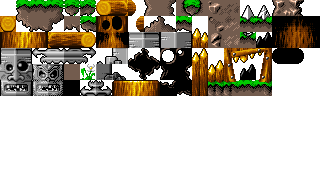
\includegraphics[width=.9\linewidth]{./graphics/tiles/area02_level_tiles.png}

Each frame of this tileset is 16��16 pixels. Load it up with a method you should already know - Image\#load$_{\text{tiles}}$. Do it in SceneMap\#initialize:

\lstset{language=Ruby,label= ,caption= ,numbers=none}
\begin{lstlisting}
@tileset = Image.load_tiles($window, "graphics/tiles/area02_level_tiles.png", 16, 16, true)
\end{lstlisting}

What you should notice, is that now our tilable? parameter is set at true. Since tilesets are in fact 'tilable' (placed one next to the other, with no space in between), it's better to use Gosu's tilable function. What it does is that it slightly blurs the edge of the image, making the connections between two sprites look a bit better.
Another thing that I want to notice is that until now, we only loaded a 1 dimension graphics with Image\#load$_{\text{tiles}}$ (single sprites were next to another). Our tileset is a 2d spritesheet (meaning that graphics start at \{0:0\} and go both right and down). The array returned by Image\#load$_{\text{tiles}}$ is still a one-dimensional array, with indexes incrementing. When the script goes to the end of one line, it just continues, without making a second line another 'dimension' in array. This image:

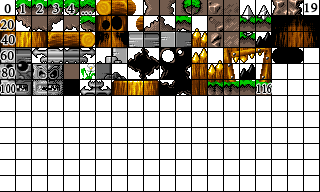
\includegraphics[width=.9\linewidth]{./graphics/tiles/area02_tileset_indexes.png}

pictures that for you.

Now it's the boring part. We have to create a new 2d array '@level[y][x]', which will hold the information about what tile is on what position. Because of our window size, we can hold 1'200 (40��30) tiles on screen at one time. But since we don't have any editor whatsoever, we have to put these values on our own. That's why, for example's sake, I'll make a smaller map. You can copy the code below to your SceneMap\#initialize:

\lstset{language=Ruby,label= ,caption= ,numbers=none}
\begin{lstlisting}
@level = []
@level[0] = [14,14,22,22,22,22,22,22,22,22,22,22,22,22,22,22,23,0,0,0,0,0,0,0,0]
@level[1] = [14,23,0,0,0,0,0,0,0,0,0,0,0,0,0,0,0,0,0,0,0,0,0,0,0]
@level[2] = [10,0,0,0,0,0,0,0,0,0,0,0,0,0,0,0,0,0,0,0,0,0,0,0,0]
@level[3] = [10,0,0,0,0,0,0,0,0,0,0,0,0,0,0,0,0,0,0,0,0,0,0,0,0]
@level[4] = [14,2,2,2,2,2,2,5,0,0,0,0,0,1,2,2,2,2,2,2,2,2,2,2,2]
@level[5] = [14,14,14,14,23,0,0,0,0,0,0,0,0,0,21,22,22,22,22,14,14,14,14,14,14]
@level[6] = [14,23,0,0,0,0,0,0,0,0,0,0,0,0,0,0,0,0,0,0,0,0,21,14,14]
@level[7] = [14,0,0,0,0,0,0,0,0,0,0,0,0,0,0,0,0,0,0,0,0,0,0,21,14]
@level[8] = [14,0,0,0,0,0,0,0,0,0,0,0,0,0,0,0,0,0,0,0,0,0,0,0,14]
@level[9] = [14,0,0,0,0,0,0,0,0,0,0,0,0,0,0,0,0,0,0,0,0,0,0,0,14]
@level[10] = [14,0,0,0,0,0,0,0,0,0,0,0,0,0,0,0,0,0,0,0,0,0,0,0,14]
@level[11] = [14,0,0,0,0,0,0,0,0,0,0,0,0,0,0,0,0,0,0,0,0,0,0,0,14]
@level[12] = [14,0,0,0,0,0,0,0,0,0,0,0,0,0,0,0,0,0,0,0,0,0,0,0,14]
@level[13] = [14,0,0,0,0,0,0,0,0,0,0,0,0,0,0,0,0,0,0,0,0,0,0,0,14]
@level[14] = [14,2,2,2,2,2,2,2,2,2,2,2,2,2,2,2,2,2,2,2,2,2,2,2,14]
\end{lstlisting}

Sorry that this level is really empty, but writing that many indices is not easy, and certainly not fun :p

We've got the simple layout of our map, now we have to display it all. In our \#draw method we'll need two 'for' loops, which will go through every field of our @level array.

\lstset{language=Ruby,label= ,caption= ,numbers=none}
\begin{lstlisting}
for y in 0...@level.size
    for x in 0...@level[y].size

    end
end
\end{lstlisting}

Good. Now two local variables - x and y - hold the indices of the graphic that is going to be displayed. Inside both loops, where I've left a blank line, type:

\lstset{language=Ruby,label= ,caption= ,numbers=none}
\begin{lstlisting}
@tileset[@level[y][x]].draw(x*16,y*16,1)
\end{lstlisting}

What does it do? It draws the correct sprite stored in @tileset array. Correct index is returned by our 2d array (@level[y][x]). Of course we have to take into account the fact that tiles are 16��16 pixels, so we have to multiply x and y by this amount. If you've done everything correctly, you should see this:

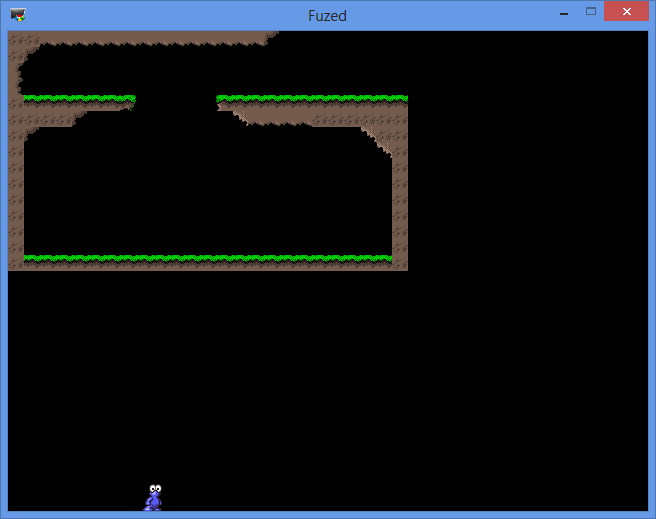
\includegraphics[width=.9\linewidth]{./pic/Level.png}

Our Player should just fall straight through it. To make it stop, we have to alter our 'SceneMap\#no$_{\text{ground}}$?' method slightly, to actually use level's data.

As you may see, in our @level array all of the empty spaces are marked by a 0. That's our 'Air' tile (empty tile), and that's exactly how we're going to treat it - if the tile our Player is on is equal to 0, he will fall. To know what tile is underneath our player, we need two variables - tile$_{\text{x}}$ and tile$_{\text{y}}$. To get the values, we'll divide our Player's x and y by 16 (tile size) and round it. So:

\lstset{language=Ruby,label= ,caption= ,numbers=none}
\begin{lstlisting}
def no_ground?(x,y)
    tile_x = (x/16).to_i
    tile_y = (y/16).to_i
end
\end{lstlisting}

Using '.to$_{\text{i'}}$ forces our variable to be an Integer. It will round the number (0 to 4 - round down, 5+ - round up). Now we just have to see if the tile we're on is 0 or not:

\lstset{language=Ruby,label= ,caption= ,numbers=none}
\begin{lstlisting}
return @level[tile_y][tile_x] == 0
\end{lstlisting}

Why '@level[tile$_{\text{y]'}}$ and not 'tile$_{\text{y}}$ + 1��? Because due to the number being rounded down, the method will always check the tile below player ;). Running the game now will show you that we'll stop on the ground. Now change our starting position to \{96:16\}. This way we'll stop on first platform:

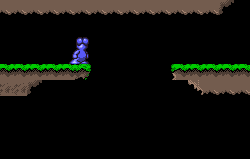
\includegraphics[width=.9\linewidth]{./pic/Platform.png}

Move right to check if we'll fall off. We will ;) so everything's correct. But if you'll keep walking in right or left, you should notice that we can walk into the wall. That's not what we need, is it? That's why we'll need a new method in SceneMap. We'll call it 'wall?', and it will take in three parameters - x, y, direction.

\lstset{language=Ruby,label= ,caption= ,numbers=none}
\begin{lstlisting}
def wall?(x,y,direction)

end
\end{lstlisting}

What is this method going to do? It's going to check if the tile next to a player (in direction we're sending in) is different than 0. So it's going to look like that:

\lstset{language=Ruby,label= ,caption= ,numbers=none}
\begin{lstlisting}
if direction == :left then
    return @level[tile_y-1][tile_x-1] != 0
elsif direction == :right then
    return @level[tile_y-1][tile_x+1] != 0
end
\end{lstlisting}

Additionally, we need to call this method every time our player moves. So our '\#update' has to be slightly changed:

\lstset{language=Ruby,label= ,caption= ,numbers=none}
\begin{lstlisting}
if $window.button_down?(KbLeft) and !wall?(@player.get_x, @player.get_y, :left) then
    @player.move_left
end
if $window.button_down?(KbRight) and !wall?(@player.get_x, @player.get_y, :right) then
    @player.move_right
end
\end{lstlisting}

Now walking into the wall will stop our character. If you'll reach the edge of the level, you'll see that we can't move anymore. That's good. But this will also create a small problem. Try jumping right after we start the game. Our Player should jump and disappear. The reason for this is that we're out of the level's border, and our code assumes that we're not in the air (tile value is nil, which is not a 0!). Even without that we would stop on the ceiling anyway. Best way to fix this is to see if there's something over our character's head. But checking this before the jump will be pointless (as after the jump the values will change), so it has to be updated every frame during the jump. Switch to the Player class, and create two new methods:

\lstset{language=Ruby,label= ,caption= ,numbers=none}
\begin{lstlisting}
def is_jumping?
    return @jump > 0
end

def reset_jump
    @jump = 0
end
\end{lstlisting}

First one will tell us if the player is in the middle of the jump; second will stop the jump immediately. Let's get back to 'SceneMap\#update' and add:

\lstset{language=Ruby,label= ,caption= ,numbers=none}
\begin{lstlisting}
if @player.is_jumping? then
    if solid_overhead?(@player.get_x, @player.get_y) then
        @player.reset_jump
    end
end
\end{lstlisting}

This bit of code is checking if the Player character is jumping, and if it is - it checks for any solid tiles above the player. If there is a tile like that, Player's jump gets cancelled. 'solid$_{\text{overhead}}$?' looks like that:

\lstset{language=Ruby,label= ,caption= ,numbers=none}
\begin{lstlisting}
def solid_overhead?(x,y)
    tile_x = (x/16).to_i
    tile_y = (y/16).to_i
    return @level[tile_y-2][tile_x] != 0
end
\end{lstlisting}

Quick test should confirm that we cannot jump out of the level anymore.

Last thing we're going to do, which is in most (if not all) of the platform games: when we'll stop pressing Up button, jumping should finish. Thanks to our '\#reset$_{\text{jump'}}$ method, it's dead easy to do. In 'SceneMap\#button$_{\text{up'}}$ add:

\lstset{language=Ruby,label= ,caption= ,numbers=none}
\begin{lstlisting}
if id == KbUp then
    @player.reset_jump if @player.is_jumping?
end
\end{lstlisting}

This method will reset Player's jump the moment Button Up is released (only if player's jumping, of course).

And that's all for today. What will next week's tutorial bring? That's a surprise ;) have fun and enjoy your week!


\section{Editor!}
\label{sec-4}
Hello all!

Today we're going to move from our game. We will be working on a basic editor for our game. This step is quite important, as it will speed up working on the game in a long run. Today we will only cover the basic map creation, and as we progress with our game, we will just add new things to it.

Word of warning before we begin: there is going to be a lot of coding. And the result won't be really exciting. But working on a game is not always cool, fun and exciting :p

Since the editor is using our game's data as well, create a new folder: '/editor'. That's where everything related to editor - both scripts and graphics - goes. Put the folder into main game's folder:

We're going to need three files as well: Editor.rb (equivalent of our Run.rb file, put it in main folder), EditorWindow.rb (equivalent of our GameWindow.rb) and SceneEditor.rb (both of these go to '/editor' folder). You should already know how to do them. The only difference is that our Editor window is going to be bigger than GameWindow - 1024��768. If your screen resolution is the same, or slightly larger, consider putting it into fullscreen, because if Gosu's window is larger than about 90\% of screen size, it's going to get scaled down. You can still use it, but the precision is a bit off.

Editor.rb:

\lstset{language=Ruby,label= ,caption= ,numbers=none}
\begin{lstlisting}
$: << File.dirname(__FILE__)

require 'gosu'
require 'rubygems'
include Gosu

require 'editor/EditorWindow.rb'
require 'editor/SceneEditor.rb'

$window = EditorWindow.new
$window.show
\end{lstlisting}

EditorWindow.rb:

\lstset{language=Ruby,label= ,caption= ,numbers=none}
\begin{lstlisting}
class EditorWindow < Gosu::Window

    def initialize
        super(1024,768,false)
        self.caption = "Fuzed: Map Editor"
        $window = self
        $scene = SceneEditor.new
    end

    def update
        $scene.update
    end

    def draw
        $scene.draw
    end

    def button_down(id)
        $scene.button_down(id)
    end

    def button_up(id)
        $scene.button_up(id)
    end

end
\end{lstlisting}

SceneEditor:

\lstset{language=Ruby,label= ,caption= ,numbers=none}
\begin{lstlisting}
class SceneEditor

    def initialize

    end

    def update

    end

    def draw

    end

    def button_down(id)

    end

    def button_up(id)

    end

end
\end{lstlisting}

We will also need a picture - background of our editor. Click here for the image.

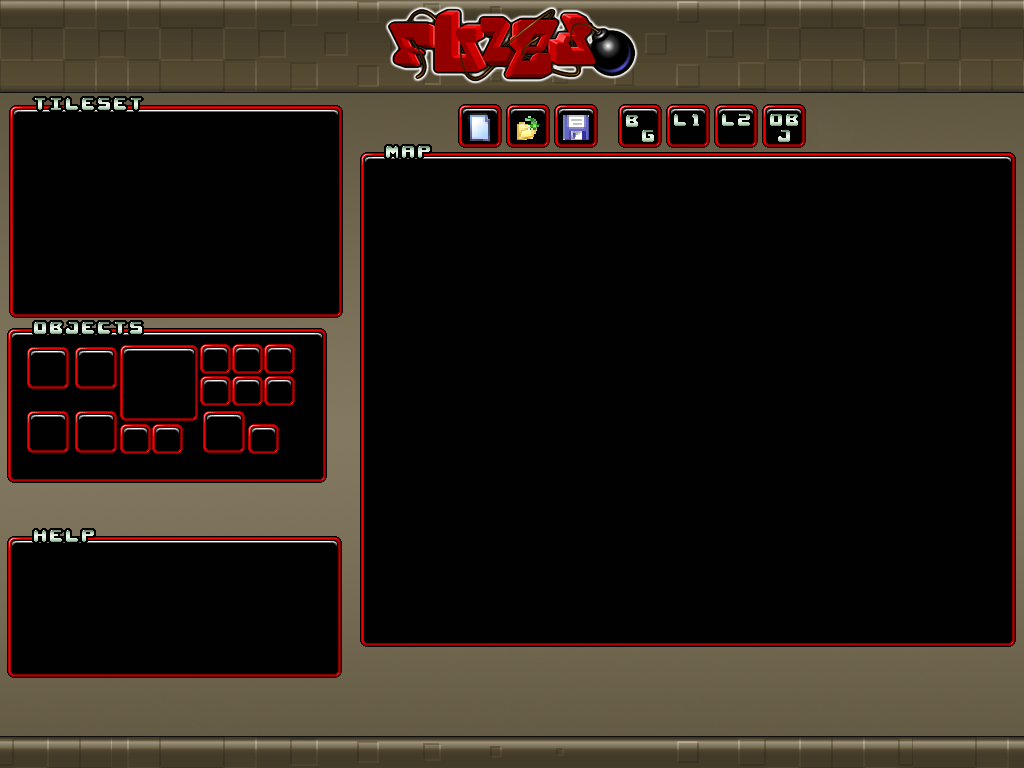
\includegraphics[width=.9\linewidth]{./editor/editor.png}

Load it up in SceneEditor as '@bg', standard image, and draw it of course ;)

\lstset{language=Ruby,label= ,caption= ,numbers=none}
\begin{lstlisting}
#initialize
@bg = Image.new($window,"editor/editor.png", false)
# draw
@bg.draw(0,0,0)
\end{lstlisting}

We are going to use mouse in our editor, but first we have to set it up. Gosu has built-in mouse support, but if you hover your mouse over the window, you'll notice that it's not there. There are two ways you can put mouse into the window: first one is to create a Cursor image and have it displayed on mouse coordinates - \$window.mouse$_{\text{x}}$, \$window.mouse$_{\text{y}}$. It will allow us to use any image we want for the cursor, but on the other hand - it's limited to game's FPS.

Second method is to allow our system cursor to be displayed on the window area. Here we're going to use this method, but if you want, you can easily use method \#1 ;)

To get our system cursor to show up on window, we need to add this method in EditorWindow:

\lstset{language=Ruby,label= ,caption= ,numbers=none}
\begin{lstlisting}
def needs_cursor?
    return true
end
\end{lstlisting}

This displays the cursor over the window:

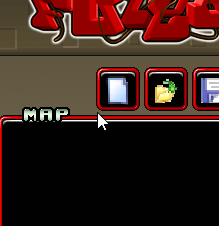
\includegraphics[width=.9\linewidth]{./pic/Cursor.png}

Next thing we have to do is to create our Map's Grid. It's going to be a 3D array. You may wonder now 'why are we going to use a 3D array in 2D game?'. Because we're going to add map layers!

At now, our map is going to have a set size, but in the future it will change ;)

\lstset{language=Ruby,label= ,caption= ,numbers=none}
\begin{lstlisting}
width = 60
height = 45
@level = []
for layer in 0...2
    @level[layer] = []
    for y in 0...height
        @level[layer][y] = []
        for x in 0...width
            @level[layer][y][x] = 0
        end
    end
end
\end{lstlisting}

This code goes to SceneEditor\#initialize. Quick explanation - For each of the layers (2 layers at the moment) we're creating an 60��45 array filled with 0. This is our, empty for now, level. We also need to load up our tileset:

\lstset{language=Ruby,label= ,caption= ,numbers=none}
\begin{lstlisting}
@tileset = Image.load_tiles($window, "graphics/tiles/area02_level_tiles.png", 16, 16, true)
\end{lstlisting}

At first lets draw our Map in the proper area, just to see if everything's working fine. In \#draw we have to add this stacked for loop:

\lstset{language=Ruby,label= ,caption= ,numbers=none}
\begin{lstlisting}
for l in 0...@level.size
    for y in 0...@level[l].size
        for x in 0...@level[l][y].size

        end
    end
end
\end{lstlisting}

Before we'll draw in our map, we have to calculate \{x;y\} of each tile. Notice that our map doesn't start at \{0;0\}, it starts at \{368;160\} instead. So this code:

\lstset{language=Ruby,label= ,caption= ,numbers=none}
\begin{lstlisting}
tx = 368 + (x*16)
ty = 160 + (y*16)
i = @level[l][y][x]
@tileset[i].draw(tx,ty,1+l)
\end{lstlisting}

Will calculate the correct position of each tile (both x, y and z). Running the editor now won't display anything, because our map is full of transparent squares. That's why, just to test it, in \#initialize change 0 to 1 when we're assigning Tile Value. Now test it. It should work, but you will notice a problem:

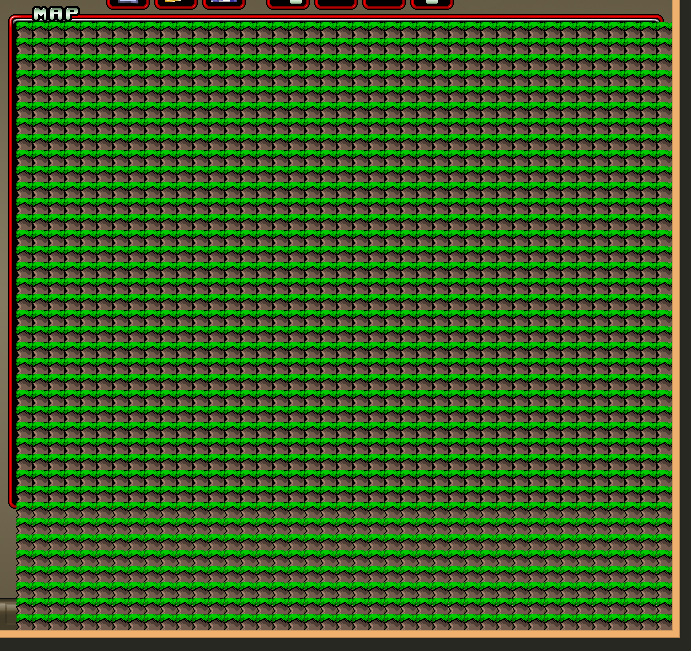
\includegraphics[width=.9\linewidth]{./pic/Test_Displayed.png}

Tiles are going outside the edges! What to do now?

Limit the loops ;) with our window size, we can display only 40��30 tiles. So:

\lstset{language=Ruby,label= ,caption= ,numbers=none}
\begin{lstlisting}
if x < 40 and y < 30 then
    tx = 368 + (x*16)
    ty = 160 + (y*16)
    i = @level[l][y][x]
    @tileset[i].draw(tx,ty,1+l)
end
\end{lstlisting}

This method will also take off a bit of load from our processor, as we won't display anything we don't need. To speed it up even more, add:

\lstset{language=Ruby,label= ,caption= ,numbers=none}
\begin{lstlisting}
if i != 0
\end{lstlisting}

At the end of '@tileset[i].draw(tx,ty,1+l)'. This will only draw tiles that are not empty (transparent tile is still there, and drawing it takes a tiny bit of the processor). You can set our tile back to 0, we've checked what we needed. Now we have to draw our tileset graphic. That may be slightly more difficult, because we have to draw a 1D array of images in 2 Dimensions. The graphic starts at \{16;112\}.

\lstset{language=Ruby,label= ,caption= ,numbers=none}
\begin{lstlisting}
for i in 0...@tileset.size
    tx = 16 + (i*16)
    ty = 112
    @tileset[i].draw(tx,ty,1)
end
\end{lstlisting}

This code will draw everything as a horizontal line, while this:

\lstset{language=Ruby,label= ,caption= ,numbers=none}
\begin{lstlisting}
for i in 0...@tileset.size
    tx = 16 + (i*16)
    ty = 112 + (i*16)
    @tileset[i].draw(tx,ty,1)
end
\end{lstlisting}

will draw it diagonally. So how do we make it so that graphic will loop back to next line each 20 tiles? Like that:

\lstset{language=Ruby,label= ,caption= ,numbers=none}
\begin{lstlisting}
for i in 0...@tileset.size
    tx = 16 + ((i%20)*16)
    ty = 112 + ((i/20)*16)
    @tileset[i].draw(tx,ty,1)
end
\end{lstlisting}

That's the first time ever we've used a Mod operator \%. This calculation will return the remainder of a division (ex. 5 \% 2 will return 1). So how does this piece of code work?

We're calculating our tx (tile x position) for tiles with mod between 0-19 (i\%20) multiplied by 16 (tile size). To calculate ty (tile y position) we're only dividing current index i by 20. With these two calculations, we should end up with:

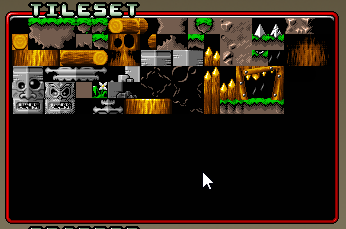
\includegraphics[width=.9\linewidth]{./pic/Tileset.png}

Next thing we have to do is mouse controls. We'll start off with detecting a mouse click, then checking where did we click, and we'll finish with selecting a tile and placing it on a map :) in SceneEditor\#button$_{\text{down}}$ put a if statement checking whether we pressed a left mouse button:

\lstset{language=Ruby,label= ,caption= ,numbers=none}
\begin{lstlisting}
if id == MsLeft then
    click
end
\end{lstlisting}

This, as you can see, sends us to 'click' method that doesn't exist. Create it, and put two ifs, checking whether we've clicked somewhere over tileset or map. To do that, we'll use Ruby's method: \#between():

\lstset{language=Ruby,label= ,caption= ,numbers=none}
\begin{lstlisting}
def click
    if $window.mouse_x.between?(16, 336) and $window.mouse_y.between?(112, 304) then
        p "tileset"
    elsif $window.mouse_x.between?(368, 1008) and $window.mouse_y.between?(160, 640) then
        p "map"
    end
end
\end{lstlisting}

Now if you were to test it, you should notice that pressing left mouse button over these two sections of the editor will print correct words into the command window. Since this works, we'll now work on selecting the tile. We will use this graphic:


\includegraphics[width=.9\linewidth]{./editor/sel16.png}

to mark the tile that is currently selected. Load this as an image into '@sel$_{\text{16'}}$ variable. Create two additional variables as well: @sel$_{\text{16}}$$_{\text{x}}$ and @sel$_{\text{16}}$$_{\text{y}}$. The values of these variables should be immediately set to 16 and 112, so frame will get displayed over first tile. Create another variable: '@selected$_{\text{tile}}$ = 0'.

\lstset{language=Ruby,label= ,caption= ,numbers=none}
\begin{lstlisting}
#Initialize
@sel_16 = Image.new($window, "editor/sel16.png", false)
@sel_16_x = 16
@sel_16_y = 112
@selected_tile = 0

# Draw
@sel_16.draw(@sel_16_x, @sel_16_y, 5
\end{lstlisting}

Now, the easy part is done. Now its time for selecting the tile. In our SceneEditor\#click method, replace 'p "tileset"' with:

\lstset{language=Ruby,label= ,caption= ,numbers=none}
\begin{lstlisting}
select_tile($window.mouse_x, $window.mouse_y)
\end{lstlisting}

And of course, create this method ('select$_{\text{tile}}$(mouseX, mouseY)'):

\lstset{language=Ruby,label= ,caption= ,numbers=none}
\begin{lstlisting}
def select_tile(x,y)
    tx = ((x - 16) / 16).floor
    ty = ((y - 112) / 16).floor
    i = tx + (ty*20)
    @sel_16_x = (tx * 16) + 16
    @sel_16_y = (ty * 16) + 112
    @select_tile = i
end
\end{lstlisting}

This code calculates our mouse X and Y and turns them into tile X and tile Y by subtracting the start of tileset graphic, dividing by tile size and rounding it down. If we were to use '.to$_{\text{i'}}$, clicking over right or bottom side of the tile would select completely different one. Next it calculates the index of selected tile. Then it calculates the position of our Selected frame and saves everything. Why did I calculate these positions (@sel$_{\text{16}}$$_{\text{x}}$/y) instead of using x and y from parameters? Because they wouldn't be aligned to the frame.

Next thing we have to do is to create a 'place$_{\text{tile}}$(x,y) method and put it in place of 'p "map"'. It's going to accept the same data as the method above - mouse x and y position. Also, create a new variable in \#initialize - @current$_{\text{layer}}$ = 0.

Placing the tile is going to be quite simple. We will calculate tx and ty (position of the tile), and then we will change the correct value in our @level variable. It's pretty simple, you can do it yourself easily ;)

\lstset{language=Ruby,label= ,caption= ,numbers=none}
\begin{lstlisting}
def place_tile(x,y)
    tx = ((x - 368) / 16).floor
    ty = ((y - 160) / 16).floor
    @level[@current_layer][ty][tx] = @select_tile
end
\end{lstlisting}

Now you can see that we can place our tiles on the map. But it's only one tile per click! Let's head to our \#update method and add:

\lstset{language=Ruby,label= ,caption= ,numbers=none}
\begin{lstlisting}
if $window.button_down?(MsLeft) and $window.mouse_x.between?(368, 1008) and $window.mouse_y.between?(160, 640) then
    place_tile($window.mouse_x, $window.mouse_y)
end
\end{lstlisting}

Now we can 'draw' on a map with tiles. Try it yourself, select a tile and draw all over the wind\ldots{}

Error

\ldots{}oh.

As we can read from the error message, there seems to be problem with reading an Integer from a nil value. What does it mean? That we're sending no data where an Integer is expected. Let's go to the line of code where this error occurs (line 69 in my code).

\lstset{language=Ruby,label= ,caption= ,numbers=none}
\begin{lstlisting}
@tileset[i].draw(tx,ty,1+l) if i != 0
\end{lstlisting}

That's the line. We have to 'nil-proof' it. Add another condition in the end of the line:

\lstset{language=Ruby,label= ,caption= ,numbers=none}
\begin{lstlisting}
@tileset[i].draw(tx,ty,1+l) if i != 0 and i != nil
\end{lstlisting}

And\ldots{} et viola! Now we can actually work on our map!

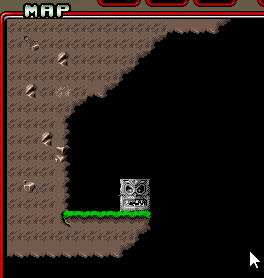
\includegraphics[width=.9\linewidth]{./pic/Map.png}

(it's not the best I could do, but wel\ldots{} :p). Seems we're almost done? Not exactly, there's still few things we have to do. Start off with saving and loading up this image:

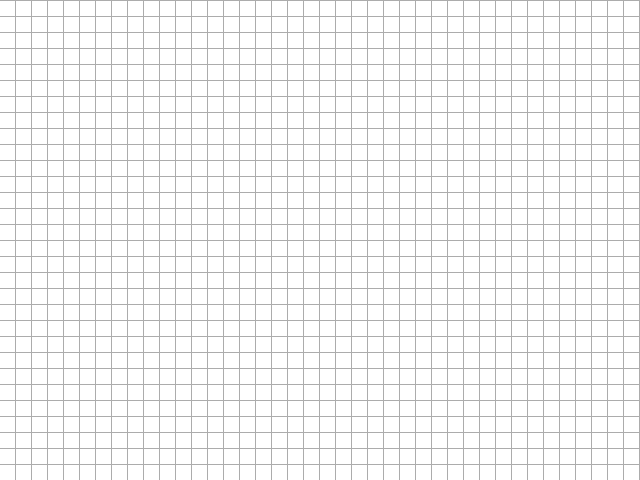
\includegraphics[width=.9\linewidth]{./editor/grid.png}

It's going to be displayed over Map area, so we see the tile edges better. Display this graphic on \{368;160;5\}.

We still have to do 4 things here: Scrolling the map, toggling between layers, placing our player's starting position and, of course, saving it to a file.

Let us start with creating three new variables:

\lstset{language=Ruby,label= ,caption= ,numbers=none}
\begin{lstlisting}
@offset_x = 0
@offset_y = 0
@ctrl_held = false
\end{lstlisting}

First two will hold our offset, which is the amount of tiles our map has been scrolled in given direction. The last one will be useful when scrolling. Now head to \#button$_{\text{down}}$ and add three ifs:

\lstset{language=Ruby,label= ,caption= ,numbers=none}
\begin{lstlisting}
if id == MsWheelDown then
    increase_offset
end
if id == MsWheelUp then
    decrease_offset
end
if id == KbLeftControl then
    @ctrl_held = true
end
\end{lstlisting}

Third 'if' should go to \#button$_{\text{up}}$ as well, with only difference being that we change the value of variable to false. Lets create the missing methods too:

\lstset{language=Ruby,label= ,caption= ,numbers=none}
\begin{lstlisting}
def increase_offset
    if @ctrl_held then
        @offset_x += 1
    else
        @offset_y += 1
    end
end

def decrease_offset
    if @ctrl_held then
        @offset_x -= 1
    else
        @offset_y -= 1
    end
end
\end{lstlisting}

There's what we've done and how does it work. Whenever we use our scroll wheel, our @offset$_{\text{y}}$ changes. But if we're using scroll wheel while holding down left control, @offset$_{\text{x}}$ changes instead. Now we'll put a few conditions too, to don't allow offsets below 0 and greater than map size - visible area. This way we'll be sure our map doesn't go missing somewhere far out of borders ;) Last thing is to actually create a visual effect from our offsets. We'll start off with the latter. In \#draw, find this piece of code:

\lstset{language=Ruby,label= ,caption= ,numbers=none}
\begin{lstlisting}
i = @level[l][y][x]
\end{lstlisting}

And change it to

\lstset{language=Ruby,label= ,caption= ,numbers=none}
\begin{lstlisting}
i = @level[l][y + @offset_y][x + @offset_x]
\end{lstlisting}

Run the game now, place a tile and try it yourself. The problem may rise if you don't have a mouse with scroll wheel, or you're using a laptop. For that, we'll change the method to work with arrow buttons. Add a parameter 'forced = false' to both methods changing offsets, and change them into:

\lstset{language=Ruby,label= ,caption= ,numbers=none}
\begin{lstlisting}
def increase_offset(forced = false)
    if @ctrl_held or forced then
        @offset_x += 1 if (@offset_x < @level[0][0].size - 40)
    else
        @offset_y += 1 if (@offset_y 0
                       else
                           @offset_y -= 1 if @offset_y > 0
                       end
end
\end{lstlisting}

You can see that I've also added the conditions keeping the map in the area. Now we just have to add Arrows to \#button$_{\text{down}}$ method:

\lstset{language=Ruby,label= ,caption= ,numbers=none}
\begin{lstlisting}
if id == KbUp then
    decrease_offset
end
if id == KbDown then
    increase_offset
end
if id == KbLeft then
    decrease_offset(true)
end
if id == KbRight then
    increase_offset(true)
end
\end{lstlisting}

"Forced" parameter, as you might already noticed, is used only with left and right arrow buttons. Yup, you guessed it right - works exactly the same as pressing left control, without actually doing it. But the other way works too ;). Now we have to do one more fix. Run your editor, place a tile, scroll the map a little bit, and place another tile - you'll notice it appeared somewhere else. That's because we don't consider offsets when placing tiles. Yet. But you can fix it yourself - just add both offsets to tx and ty in \#place$_{\text{tile}}$ method. When it's done, everything should work just fine.

Now let's do our Layers. We will need this graphic:

We're using it exactly the same way as we used '@sel$_{\text{16'}}$ (but it's 32 this time). Starting position is \{672:112\}, and when drawing, put it at z = 5.

Now alter our \#click function, to check for layer buttons as well:

\lstset{language=Ruby,label= ,caption= ,numbers=none}
\begin{lstlisting}
elsif $window.mouse_x.between?(672,704) and $window.mouse_y.between?(112,144) then
    @current_layer = 0
    @sel_32_x = 672
elsif $window.mouse_x.between?(720,752) and $window.mouse_y.between?(112,144) then
    @current_layer = 1
    @sel_32_x = 720
\end{lstlisting}

Now to actually distinguish between active and inactive layer, we have to go to \#draw. The easiest thing to do is to change the opacity of inactive layer to 160. This code:

\lstset{language=Ruby,label= ,caption= ,numbers=none}
\begin{lstlisting}
@tileset[i].draw(tx,ty,1+l) if i != 0 and i != nil
\end{lstlisting}

Has to be slightly expanded. Start off with putting an if statement to check, if Layer l is active or not:

\lstset{language=Ruby,label= ,caption= ,numbers=none}
\begin{lstlisting}
if l == @current_layer then

else

end
\end{lstlisting}

And we'll expand our drawing code. Gosu::Image\#draw can take more than 3 parameters:

\lstset{language=Ruby,label= ,caption= ,numbers=none}
\begin{lstlisting}
draw(x, y, z, scale_x, scale_y, color, mode)
\end{lstlisting}

scale$_{\text{x}}$/$_{\text{y}}$ are simple enough. They default to 1.0 if we don't give any value, and that's what we'll have to put there (so the image size won't change). It's the color value that interests us the most. We don't change a thing for the active layer, but for the other layer(s) (below 'else'), we'll have to change the color to Color.new(160,255,255,255):

\lstset{language=Ruby,label= ,caption= ,numbers=none}
\begin{lstlisting}
@tileset[i].draw(tx,ty,1+l,1.0,1.0,Color.new(160,255,255,255)) if i != 0 and i != nil
\end{lstlisting}

Give it a try - place few tiles on first layer and then change the layer to second one. It will turn slightly transparent. You can change the amount of transparency yourself.

Now we'll work on placing our Player. We need few more variables for that:

\lstset{language=Ruby,label= ,caption= ,numbers=none}
\begin{lstlisting}
@objects = []
@player_graphic = Image.load_tiles($window, "graphics/sprites/player_1_run_left.png", 32, 32, false)
@active_mode = :map
@object_held = nil
\end{lstlisting}

'@active$_{\text{mode'}}$ is the important one. It's the variable we'll use to check if we are placing tiles, or objects (player, with more objects coming in the future). Let's draw our player too:

\lstset{language=Ruby,label= ,caption= ,numbers=none}
\begin{lstlisting}
frame = milliseconds / 150 % @player_graphic.size
@player_graphic[frame].draw(32,352,1)
\end{lstlisting}

And check for click in this area (\{32;352\}, size is 32��32). If we do, we'll call a 'select$_{\text{object}}$(:player)' method, in which we'll assign a value to @object$_{\text{held}}$ variable and we'll change the mode to :objects.

\lstset{language=Ruby,label= ,caption= ,numbers=none}
\begin{lstlisting}
def select_object(object)
@object_held = object
@active_mode = :objects
@sel_32_x = 768
end
\end{lstlisting}

Now go to \#draw and add:

\lstset{language=Ruby,label= ,caption= ,numbers=none}
\begin{lstlisting}
case @object_held
when nil

when :player
    @player_graphic[0].draw($window.mouse_x, $window.mouse_y,10)
end
\end{lstlisting}

That's a Switch (or Case) statement, which we'll use from time to time. This one will draw a graphic of our player under a mouse cursor whenever we've selected our player.

Now since we've got selecting, it's time to place the player. Go back to \#click method, and change the bit where it calls \#place$_{\text{tile}}$ to this:

\lstset{language=Ruby,label= ,caption= ,numbers=none}
\begin{lstlisting}
if @active_mode == :map then
   place_tile($window.mouse_x, $window.mouse_y)
elsif @active_mode == :objects then
   place_object($window.mouse_x, $window.mouse_y)
end
\end{lstlisting}

Add the method too:

\lstset{language=Ruby,label= ,caption= ,numbers=none}
\begin{lstlisting}
def place_object(x,y)
    rx = x + (@offset_x*16) - 368
    ry = y + (@offset_y*16) - 160
    @objects << [@object_held, rx, ry]
    if @object_held == :player then
        @object_held = nil
    end
end
\end{lstlisting}

This code will add Player's starting position, and (in this case), change object currently held to nil, so we won't "draw" a line of players. We won't do that with other types of objects. Now we have to display these objects on our map:

\lstset{language=Ruby,label= ,caption= ,numbers=none}
\begin{lstlisting}
for i in 0...@objects.size
    case @objects[i][0]
    when :player
        frame = milliseconds / 150 % @player_graphic.size
        rx = @objects[i][1] - (@offset_x * 16) + 368
        ry = @objects[i][2] - (@offset_y * 16) + 160
        @player_graphic[frame].draw(rx,ry,6)
    end
end
\end{lstlisting}

Now you can place our player on the map. But if you'll place it again, you may notice that we've got two players. We have to do something about that. Let's go back to \#place$_{\text{object}}$ and put this on the top:

\lstset{language=Ruby,label= ,caption= ,numbers=none}
\begin{lstlisting}
if @object_held == :player then
    for i in 0...@objects.size
        if @objects[i][0] == :player
            @objects.delete_at(i)
        end
    end
end
\end{lstlisting}

This will check if our @objects array already contains a player. If it does, it will remove it first before placing another one. And before we'll go to the last part of today's tutorial, go to \#select$_{\text{tile}}$ method and add:

\lstset{language=Ruby,label= ,caption= ,numbers=none}
\begin{lstlisting}
@active_mode = :map
\end{lstlisting}

so the mode changes back when creating map. And now to saving!

First check for mouse click over \{560;112\} (save icon), which will call the \#save method.

Our file will have to hold three pieces of data - the map itself, which tileset we're using and all objects we're using. For now we'll save our map as "Map000.map". This will change in future ;)

Our \#save method:

\lstset{language=Ruby,label= ,caption= ,numbers=none}
\begin{lstlisting}
def save
    f = File.new("Map000.map", "w+")
    Marshal.dump(@tileset, f)
    Marshal.dump(@level, f)
    Marshal.dump(@objects, f)
    f.close
end
\end{lstlisting}

Marshal is a Ruby's class that allows us to save variables into file. The method is fairly straightforward - we're creating a new File, put data into it, and close the file. But\ldots{}

Marshal error

The reason for that is Ruby's Marhsal has no idea what a Gosu::Image is. We can only save tileset's path/to/file as a string. That's why in our \#initialize, add this variable:

\lstset{language=Ruby,label= ,caption= ,numbers=none}
\begin{lstlisting}
@used_tileset = "area02_level_tiles.png"
\end{lstlisting}

And change:

\lstset{language=Ruby,label= ,caption= ,numbers=none}
\begin{lstlisting}
@tileset = Image.load_tiles($window, "graphics/tiles/#{@used_tileset}", 16, 16, true)
\end{lstlisting}

And change '@tileset' to '@used$_{\text{tileset'}}$ in \#save method too. Now, pressing the Save button in editor will create\ldots{}

Saved file

This! =)

And that's it for today! We've done quite a bit of work :) in next tutorial we will work on actually loading up the map into the game, and working with a map bigger than the screen. And then\ldots{} we'll see ;)

\section{4.5 (Special 1): Parsing maps from Tiled (optional).}
\label{sec-5}
\section{Camera.}
\label{sec-6}
\section{Fixes and improvements!}
\label{sec-7}
\section{Diamonds!}
\label{sec-8}
\section{Invulnerability, sounds and\ldots{}}
\label{sec-9}
\section{References}
\label{sec-10}
\begin{itemize}
\item \url{https://corruptgd.wordpress.com/tutorials-creating-a-platformer-in-ruby-gosu/}
\end{itemize}
% Emacs 24.3.1 (Org mode 8.2.7c)
\end{document}